\begin{figure}[H]
			\centering		
			\begin{tikzpicture}
				\pgfmathsetmacro{\cubex}{0.01}
				\pgfmathsetmacro{\cubey}{5}
				\pgfmathsetmacro{\cubez}{5}
				
				\begin{scope}[line width=0.2mm]
				\begin{scope}
				\clip[] (-0.8,0,0) -- ++(-\cubex,0,0) -- ++(0,-\cubey,0) -- ++(\cubex,0,0) -- cycle;
				\draw[fill=white] (-0.8,0,0) -- ++(-\cubex,0,0) -- ++(0,-\cubey,0) -- ++(\cubex,0,0) -- cycle;
				\end{scope}
				\begin{scope}
				\clip[] (-0.8,0,0) -- ++(0,0,-\cubez) -- ++(0,-\cubey,0) -- ++(0,0,\cubez) -- cycle;
				\draw[fill=white] (-0.8,0,0) -- ++(0,0,-\cubez) -- ++(0,-\cubey,0) -- ++(0,0,\cubez) -- cycle;
				\end{scope}
				\begin{scope}
				\clip[] (-0.8,0,0) -- ++(-\cubex,0,0) -- ++(0,0,-\cubez) -- ++(\cubex,0,0) -- cycle;
				\draw[fill=white] (-0.8,0,0) -- ++(-\cubex,0,0) -- ++(0,0,-\cubez) -- ++(\cubex,0,0) -- cycle;
				\end{scope}
				
				\begin{scope}
				\clip[] (-0.7,0,0) -- ++(-\cubex,0,0) -- ++(0,-\cubey,0) -- ++(\cubex,0,0) -- cycle;
				\draw[fill=white] (-0.7,0,0) -- ++(-\cubex,0,0) -- ++(0,-\cubey,0) -- ++(\cubex,0,0) -- cycle;
				\end{scope}
				\begin{scope}
				\clip[] (-0.7,0,0) -- ++(0,0,-\cubez) -- ++(0,-\cubey,0) -- ++(0,0,\cubez) -- cycle;
				\draw[fill=white] (-0.7,0,0) -- ++(0,0,-\cubez) -- ++(0,-\cubey,0) -- ++(0,0,\cubez) -- cycle;
				\end{scope}
				\begin{scope}
				\clip[] (-0.7,0,0) -- ++(-\cubex,0,0) -- ++(0,0,-\cubez) -- ++(\cubex,0,0) -- cycle;
				\draw[fill=white] (-0.7,0,0) -- ++(-\cubex,0,0) -- ++(0,0,-\cubez) -- ++(\cubex,0,0) -- cycle;
				\end{scope}
			
				\begin{scope}
					\clip[] (-0.6,0,0) -- ++(-\cubex,0,0) -- ++(0,-\cubey,0) -- ++(\cubex,0,0) -- cycle;
					\draw[fill=white] (-0.6,0,0) -- ++(-\cubex,0,0) -- ++(0,-\cubey,0) -- ++(\cubex,0,0) -- cycle;
				\end{scope}
				\begin{scope}
					\clip[] (-0.6,0,0) -- ++(0,0,-\cubez) -- ++(0,-\cubey,0) -- ++(0,0,\cubez) -- cycle;
					\draw[fill=white] (-0.6,0,0) -- ++(0,0,-\cubez) -- ++(0,-\cubey,0) -- ++(0,0,\cubez) -- cycle;
				\end{scope}
				\begin{scope}
					\clip[] (-0.6,0,0) -- ++(-\cubex,0,0) -- ++(0,0,-\cubez) -- ++(\cubex,0,0) -- cycle;
					\draw[fill=white] (-0.6,0,0) -- ++(-\cubex,0,0) -- ++(0,0,-\cubez) -- ++(\cubex,0,0) -- cycle;
				\end{scope}	
				
				\begin{scope}
					\node[rotate=-22] (png) at (0.35,-1.8) {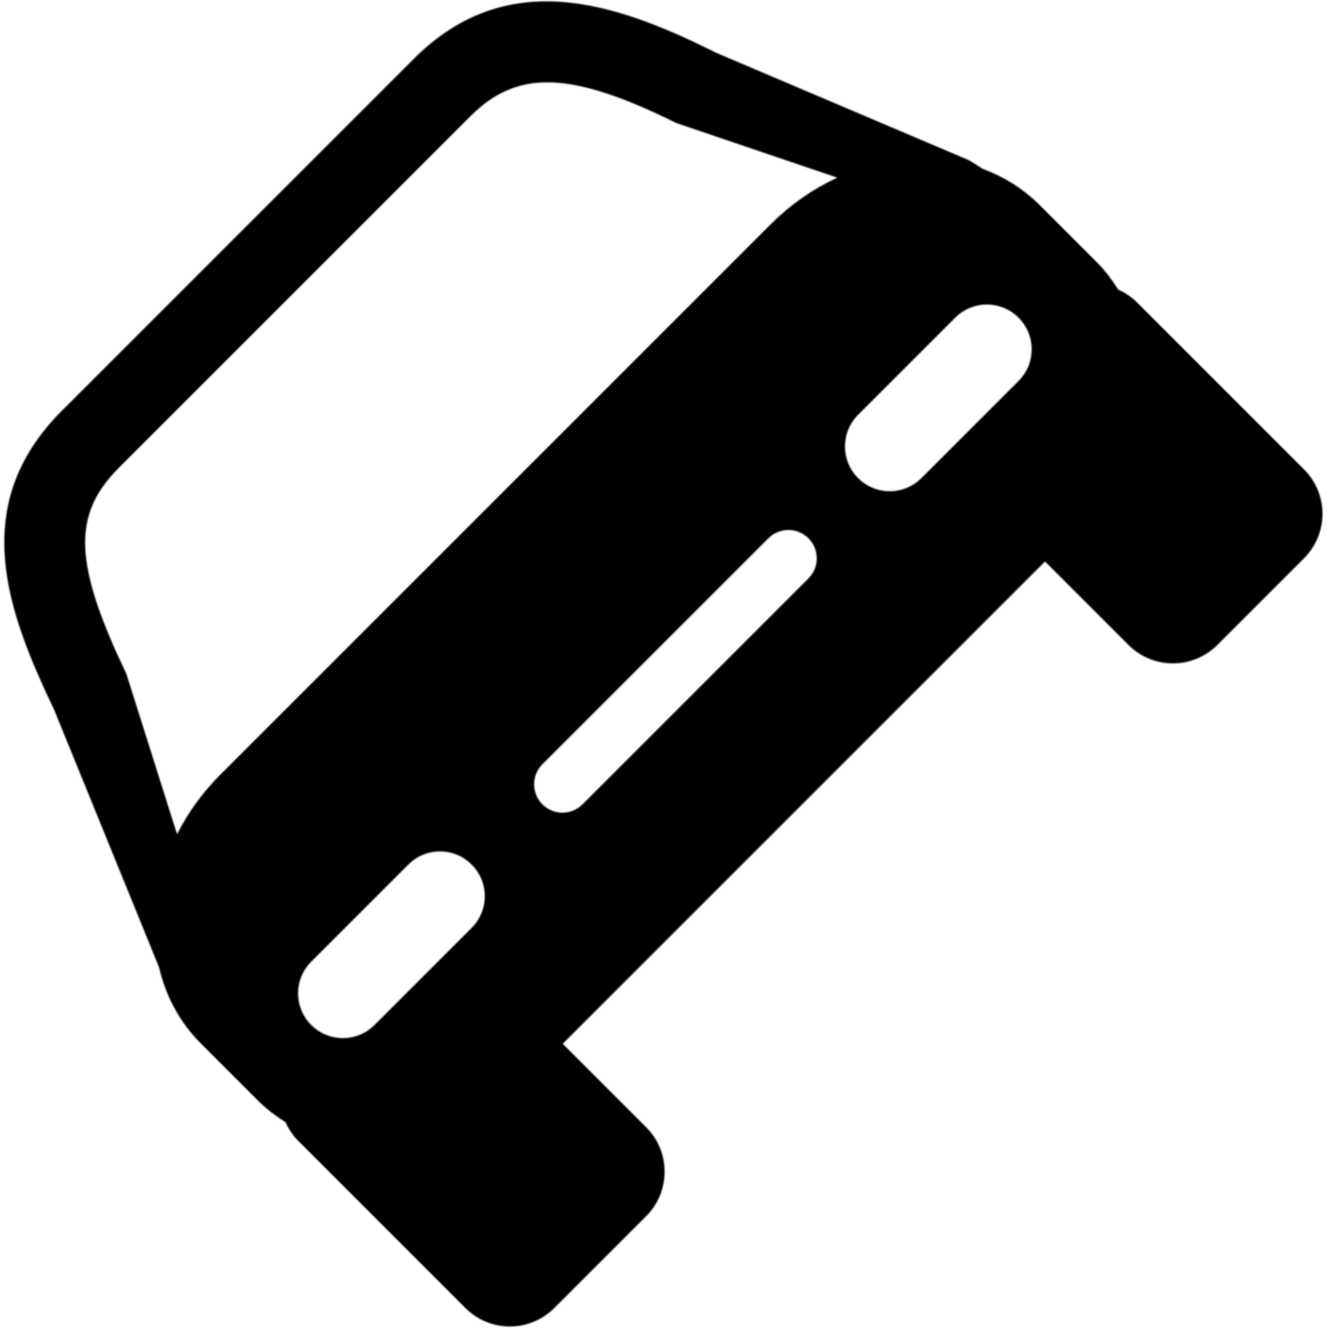
\includegraphics[height=3cm, width=1.5cm]{Bilder/png.png}};
				\end{scope}
				
				\pgfmathsetmacro{\cubey}{1}
				\pgfmathsetmacro{\cubez}{1}
				\pgfmathsetmacro{\x}{0.3}
				\pgfmathsetmacro{\y}{-2.3}
				
				\begin{scope}
					\clip[] (\x,\y,0) -- ++(0,0,-\cubez) -- ++(0,-\cubey,0) -- ++(0,0,\cubez) -- cycle;
					\draw[fill=white] (\x,\y,0) -- ++(0,0,-\cubez) -- ++(0,-\cubey,0) -- ++(0,0,\cubez) -- cycle;
				\end{scope}
				
				\draw[] (\x,\y-0.014,0) -- (1.809,-2.299,0);
				\draw[] (\x-0.002,\y-0.014,-\cubez) -- (1.801,-2.312,-0.5);
				\draw[] (\x-0.003,\y+0.005-\cubey,-\cubez) -- (1.799,-2.289-0.5,-0.5);
				\draw[] (\x+0.002,\y+0.009-\cubey,0) -- (1.805,-2.286-0.5,0);
				
				\pgfmathsetmacro{\cubey}{0.5}
				\pgfmathsetmacro{\cubez}{0.5}
				\pgfmathsetmacro{\x}{1.8}
				\pgfmathsetmacro{\y}{-2.3}
				
				\begin{scope}
					\clip[] (\x,\y,0) -- ++(0,0,-\cubez) -- ++(0,-\cubey,0) -- ++(0,0,\cubez) -- cycle;
					\draw[] (\x,\y,0) -- ++(0,0,-\cubez) -- ++(0,-\cubey,0) -- ++(0,0,\cubez) -- cycle;
				\end{scope}
				
				
				
				\pgfmathsetmacro{\cubex}{2}
				\pgfmathsetmacro{\cubey}{3}
				\pgfmathsetmacro{\cubez}{3}
				\pgfmathsetmacro{\x}{3.6}
				\pgfmathsetmacro{\y}{-0.5}
				
				\begin{scope}
					\clip[] (\x,\y,0) -- ++(-\cubex,0,0) -- ++(0,-\cubey,0) -- ++(\cubex,0,0) -- cycle;
					\draw[] (\x,\y,0) -- ++(-\cubex,0,0) -- ++(0,-\cubey,0) -- ++(\cubex,0,0) -- cycle;
				\end{scope}
				\begin{scope}
					\clip[] (\x,\y,0) -- ++(0,0,-\cubez) -- ++(0,-\cubey,0) -- ++(0,0,\cubez) -- cycle;
					\draw[] (\x,\y,0) -- ++(0,0,-\cubez) -- ++(0,-\cubey,0) -- ++(0,0,\cubez) -- cycle;
				\end{scope}
				\begin{scope}
					\clip[] (\x,\y,0) -- ++(-\cubex,0,0) -- ++(0,0,-\cubez) -- ++(\cubex,0,0) -- cycle;
					\draw[] (\x,\y,0) -- ++(-\cubex,0,0) -- ++(0,0,-\cubez) -- ++(\cubex,0,0) -- cycle;
				\end{scope}	
				\begin{scope}
					\clip[] (\x,\y,0-\cubez) -- ++(-\cubex,0,0) -- ++(0,-\cubey,0) -- ++(\cubex,0,0) -- cycle;
					\draw[] (\x,\y,0-\cubez) -- ++(-\cubex,0,0) -- ++(0,-\cubey,0) -- ++(\cubex,0,0) -- cycle;
				\end{scope}	
				\begin{scope}
					\clip[] (\x,\y-\cubey,0) -- ++(-\cubex,0,0) -- ++(0,0,-\cubez) -- ++(\cubex,0,0) -- cycle;
					\draw[] (\x,\y-\cubey,0) -- ++(-\cubex,0,0) -- ++(0,0,-\cubez) -- ++(\cubex,0,0) -- cycle;
				\end{scope}	
			
				\pgfmathsetmacro{\cubey}{1}
				\pgfmathsetmacro{\cubez}{1}
				\pgfmathsetmacro{\x}{3.8}
				\pgfmathsetmacro{\y}{-2}
				
				\begin{scope}
					\clip[] (\x,\y,0) -- ++(0,0,-\cubez) -- ++(0,-\cubey,0) -- ++(0,0,\cubez) -- cycle;
					\draw[] (\x,\y,0) -- ++(0,0,-\cubez) -- ++(0,-\cubey,0) -- ++(0,0,\cubez) -- cycle;
					
				\end{scope}
					\draw[] (\x-0.003,\y-0.01,0) -- (7.16,-2.01,0);
					\draw[] (\x,\y-0.02,-\cubez) -- (7.165,-1.999,-0.2);
					\draw[] (\x-0.005,\y-0.00-\cubey,-\cubez) -- (7.165,-2.02-0.2,-0.2);
					\draw[] (\x-0.001,\y+0.001-\cubey,0) -- (7.165,-2.02-0.2,0);
					
					
				\pgfmathsetmacro{\cubex}{2}
				\pgfmathsetmacro{\cubey}{2}
				\pgfmathsetmacro{\cubez}{2}
				\pgfmathsetmacro{\x}{7}
				\pgfmathsetmacro{\y}{-1}
				
				\begin{scope}
					\clip[] (\x,\y,0) -- ++(-\cubex,0,0) -- ++(0,-\cubey,0) -- ++(\cubex,0,0) -- cycle;
					\draw[] (\x,\y,0) -- ++(-\cubex,0,0) -- ++(0,-\cubey,0) -- ++(\cubex,0,0) -- cycle;
				\end{scope}
				\begin{scope}
					\clip[] (\x,\y,0) -- ++(0,0,-\cubez) -- ++(0,-\cubey,0) -- ++(0,0,\cubez) -- cycle;
					\draw[] (\x,\y,0) -- ++(0,0,-\cubez) -- ++(0,-\cubey,0) -- ++(0,0,\cubez) -- cycle;
				\end{scope}
				\begin{scope}
					\clip[] (\x,\y,0) -- ++(-\cubex,0,0) -- ++(0,0,-\cubez) -- ++(\cubex,0,0) -- cycle;
					\draw[] (\x,\y,0) -- ++(-\cubex,0,0) -- ++(0,0,-\cubez) -- ++(\cubex,0,0) -- cycle;
				\end{scope}	
				\begin{scope}
					\clip[] (\x,\y,0-\cubez) -- ++(-\cubex,0,0) -- ++(0,-\cubey,0) -- ++(\cubex,0,0) -- cycle;
					\draw[] (\x,\y,0-\cubez) -- ++(-\cubex,0,0) -- ++(0,-\cubey,0) -- ++(\cubex,0,0) -- cycle;
				\end{scope}	
				\begin{scope}
					\clip[] (\x,\y-\cubey,0) -- ++(-\cubex,0,0) -- ++(0,0,-\cubez) -- ++(\cubex,0,0) -- cycle;
					\draw[] (\x,\y-\cubey,0) -- ++(-\cubex,0,0) -- ++(0,0,-\cubez) -- ++(\cubex,0,0) -- cycle;
				\end{scope}
				
				\pgfmathsetmacro{\cubey}{0.25}
				\pgfmathsetmacro{\cubez}{0.25}
				\pgfmathsetmacro{\x}{7.15}
				\pgfmathsetmacro{\y}{-2}
				
				\begin{scope}
					\clip[] (\x,\y,0) -- ++(0,0,-\cubez) -- ++(0,-\cubey,0) -- ++(0,0,\cubez) -- cycle;
					\draw[] (\x,\y,0) -- ++(0,0,-\cubez) -- ++(0,-\cubey,0) -- ++(0,0,\cubez) -- cycle;
				\end{scope}
			
				\pgfmathsetmacro{\cubex}{2}
				\pgfmathsetmacro{\cubey}{0.8}
				\pgfmathsetmacro{\cubez}{0.8}
				\pgfmathsetmacro{\x}{7.35}
				\pgfmathsetmacro{\y}{-0.9}
				
				\begin{scope}
					\clip[] (\x,\y,0) -- ++(-\cubex,0,0) -- ++(0,-\cubey,0) -- ++(\cubex,0,0) -- cycle;
					\draw[] (\x,\y,0) -- ++(-\cubex,0,0) -- ++(0,-\cubey,0) -- ++(\cubex,0,0) -- cycle;
				\end{scope}
				\begin{scope}
					\clip[] (\x,\y,0) -- ++(0,0,-\cubez) -- ++(0,-\cubey,0) -- ++(0,0,\cubez) -- cycle;
					\draw[] (\x,\y,0) -- ++(0,0,-\cubez) -- ++(0,-\cubey,0) -- ++(0,0,\cubez) -- cycle;
				\end{scope}
				\begin{scope}
					\clip[] (\x,\y,0) -- ++(-\cubex,0,0) -- ++(0,0,-\cubez) -- ++(\cubex,0,0) -- cycle;
					\draw[] (\x,\y,0) -- ++(-\cubex,0,0) -- ++(0,0,-\cubez) -- ++(\cubex,0,0) -- cycle;
				\end{scope}	
				\begin{scope}
					\clip[] (\x,\y,0-\cubez) -- ++(-\cubex,0,0) -- ++(0,-\cubey,0) -- ++(\cubex,0,0) -- cycle;
					\draw[] (\x,\y,0-\cubez) -- ++(-\cubex,0,0) -- ++(0,-\cubey,0) -- ++(\cubex,0,0) -- cycle;
				\end{scope}	
				\begin{scope}
					\clip[] (\x,\y-\cubey,0) -- ++(-\cubex,0,0) -- ++(0,0,-\cubez) -- ++(\cubex,0,0) -- cycle;
					\draw[] (\x,\y-\cubey,0) -- ++(-\cubex,0,0) -- ++(0,0,-\cubez) -- ++(\cubex,0,0) -- cycle;
				\end{scope}
			
				\draw[] (\x-0.003,\y-0.015,0) -- (8.515,-1.09,0);
				\draw[] (\x-0.01,\y-0.01,-\cubez) -- (8.5,-1.115,-0.2);
				\draw[] (\x,\y-\cubey,-\cubez) -- (8.499,-1.09-0.2,-0.2);
				\draw[] (\x,\y-\cubey,0) -- (8.505,-1.085-0.2,0);
			
				\pgfmathsetmacro{\cubey}{0.2}
				\pgfmathsetmacro{\cubez}{0.2}
				\pgfmathsetmacro{\x}{8.5}
				\pgfmathsetmacro{\y}{-1.1}
				
				\begin{scope}
					\clip[] (\x,\y,0) -- ++(0,0,-\cubez) -- ++(0,-\cubey,0) -- ++(0,0,\cubez) -- cycle;
					\draw[] (\x,\y,0) -- ++(0,0,-\cubez) -- ++(0,-\cubey,0) -- ++(0,0,\cubez) -- cycle;
				\end{scope}
				
				
			
				\pgfmathsetmacro{\cubex}{0.5}
				\pgfmathsetmacro{\cubey}{0.5}
				\pgfmathsetmacro{\cubez}{0.5}
				
				
				\begin{scope}
					\clip[] (11.5,1,0) -- ++(-\cubex,0,0) -- ++(0,-\cubey,0) -- ++(\cubex,0,0) -- cycle;
					\draw[fill=white] (11.5,1,0) -- ++(-\cubex,0,0) -- ++(0,-\cubey,0) -- ++(\cubex,0,0) -- cycle;
				\end{scope}
				\begin{scope}
					\clip[] (11.5,0.5,0) -- ++(-\cubex,0,0) -- ++(0,-\cubey,0) -- ++(\cubex,0,0) -- cycle;
					\draw[fill=white] (11.5,0.5,0) -- ++(-\cubex,0,0) -- ++(0,-\cubey,0) -- ++(\cubex,0,0) -- cycle;
				\end{scope}
				\begin{scope}
					\clip[] (11.5,0,0) -- ++(-\cubex,0,0) -- ++(0,-\cubey,0) -- ++(\cubex,0,0) -- cycle;
					\draw[fill=white] (11.5,0,0) -- ++(-\cubex,0,0) -- ++(0,-\cubey,0) -- ++(\cubex,0,0) -- cycle;
				\end{scope}
				\begin{scope}
					\clip[] (11.5,-0.5,0) -- ++(-\cubex,0,0) -- ++(0,-\cubey,0) -- ++(\cubex,0,0) -- cycle;
					\draw[fill=white] (11.5,-0.5,0) -- ++(-\cubex,0,0) -- ++(0,-\cubey,0) -- ++(\cubex,0,0) -- cycle;
				\end{scope}
				\begin{scope}
					\clip[] (11.5,-1,0) -- ++(-\cubex,0,0) -- ++(0,-\cubey,0) -- ++(\cubex,0,0) -- cycle;
					\draw[fill=white] (11.5,-1,0) -- ++(-\cubex,0,0) -- ++(0,-\cubey,0) -- ++(\cubex,0,0) -- cycle;
				\end{scope}
				\begin{scope}
					\clip[] (11.5,-1.5,0) -- ++(-\cubex,0,0) -- ++(0,-\cubey,0) -- ++(\cubex,0,0) -- cycle;
					\draw[fill=white] (11.5,-1.5,0) -- ++(-\cubex,0,0) -- ++(0,-\cubey,0) -- ++(\cubex,0,0) -- cycle;
				\end{scope}
				\begin{scope}
					\clip[] (11.5,-2,0) -- ++(-\cubex,0,0) -- ++(0,-\cubey,0) -- ++(\cubex,0,0) -- cycle;
					\draw[fill=white] (11.5,-2,0) -- ++(-\cubex,0,0) -- ++(0,-\cubey,0) -- ++(\cubex,0,0) -- cycle;
				\end{scope}
				\begin{scope}
					\clip[] (11.5,-2.5,0) -- ++(-\cubex,0,0) -- ++(0,-\cubey,0) -- ++(\cubex,0,0) -- cycle;
					\draw[fill=white] (11.5,-2.5,0) -- ++(-\cubex,0,0) -- ++(0,-\cubey,0) -- ++(\cubex,0,0) -- cycle;
				\end{scope}
				\begin{scope}
					\clip[] (11.5,-4,0) -- ++(-\cubex,0,0) -- ++(0,-\cubey,0) -- ++(\cubex,0,0) -- cycle;
					\draw[fill=white] (11.5,-4,0) -- ++(-\cubex,0,0) -- ++(0,-\cubey,0) -- ++(\cubex,0,0) -- cycle;
				\end{scope}
			
				
					\begin{scope}
					\clip[] (10,1,0) -- ++(-\cubex,0,0) -- ++(0,-\cubey,0) -- ++(\cubex,0,0) -- cycle;
					\draw[fill=white] (10,1,0) -- ++(-\cubex,0,0) -- ++(0,-\cubey,0) -- ++(\cubex,0,0) -- cycle;
				\end{scope}
				\begin{scope}
					\clip[] (10,0.5,0) -- ++(-\cubex,0,0) -- ++(0,-\cubey,0) -- ++(\cubex,0,0) -- cycle;
					\draw[fill=white] (10,0.5,0) -- ++(-\cubex,0,0) -- ++(0,-\cubey,0) -- ++(\cubex,0,0) -- cycle;
				\end{scope}
				\begin{scope}
					\clip[] (10,0,0) -- ++(-\cubex,0,0) -- ++(0,-\cubey,0) -- ++(\cubex,0,0) -- cycle;
					\draw[fill=white] (10,0,0) -- ++(-\cubex,0,0) -- ++(0,-\cubey,0) -- ++(\cubex,0,0) -- cycle;
				\end{scope}
				\begin{scope}
					\clip[] (10,-0.5,0) -- ++(-\cubex,0,0) -- ++(0,-\cubey,0) -- ++(\cubex,0,0) -- cycle;
					\draw[fill=white] (10,-0.5,0) -- ++(-\cubex,0,0) -- ++(0,-\cubey,0) -- ++(\cubex,0,0) -- cycle;
				\end{scope}
				\begin{scope}
					\clip[] (10,-1,0) -- ++(-\cubex,0,0) -- ++(0,-\cubey,0) -- ++(\cubex,0,0) -- cycle;
					\draw[fill=white] (10,-1,0) -- ++(-\cubex,0,0) -- ++(0,-\cubey,0) -- ++(\cubex,0,0) -- cycle;
				\end{scope}
				\begin{scope}
					\clip[] (10,-1.5,0) -- ++(-\cubex,0,0) -- ++(0,-\cubey,0) -- ++(\cubex,0,0) -- cycle;
					\draw[fill=white] (10,-1.5,0) -- ++(-\cubex,0,0) -- ++(0,-\cubey,0) -- ++(\cubex,0,0) -- cycle;
				\end{scope}
				\begin{scope}
					\clip[] (10,-2,0) -- ++(-\cubex,0,0) -- ++(0,-\cubey,0) -- ++(\cubex,0,0) -- cycle;
					\draw[fill=white] (10,-2,0) -- ++(-\cubex,0,0) -- ++(0,-\cubey,0) -- ++(\cubex,0,0) -- cycle;
				\end{scope}
				\begin{scope}
					\clip[] (10,-2.5,0) -- ++(-\cubex,0,0) -- ++(0,-\cubey,0) -- ++(\cubex,0,0) -- cycle;
					\draw[fill=white] (10,-2.5,0) -- ++(-\cubex,0,0) -- ++(0,-\cubey,0) -- ++(\cubex,0,0) -- cycle;
				\end{scope}
				\begin{scope}
					\clip[] (10,-4,0) -- ++(-\cubex,0,0) -- ++(0,-\cubey,0) -- ++(\cubex,0,0) -- cycle;
					\draw[fill=white] (10,-4,0) -- ++(-\cubex,0,0) -- ++(0,-\cubey,0) -- ++(\cubex,0,0) -- cycle;
				\end{scope}
			
			
					\begin{scope}
					\clip[] (13,1,0) -- ++(-\cubex,0,0) -- ++(0,-\cubey,0) -- ++(\cubex,0,0) -- cycle;
					\draw[fill=white] (13,1,0) -- ++(-\cubex,0,0) -- ++(0,-\cubey,0) -- ++(\cubex,0,0) -- cycle;
				\end{scope}
				\begin{scope}
					\clip[] (13,0.5,0) -- ++(-\cubex,0,0) -- ++(0,-\cubey,0) -- ++(\cubex,0,0) -- cycle;
					\draw[fill=white] (13,0.5,0) -- ++(-\cubex,0,0) -- ++(0,-\cubey,0) -- ++(\cubex,0,0) -- cycle;
				\end{scope}
				\begin{scope}
					\clip[] (13,0,0) -- ++(-\cubex,0,0) -- ++(0,-\cubey,0) -- ++(\cubex,0,0) -- cycle;
					\draw[fill=white] (13,0,0) -- ++(-\cubex,0,0) -- ++(0,-\cubey,0) -- ++(\cubex,0,0) -- cycle;
				\end{scope}
				\begin{scope}
					\clip[] (13,-0.5,0) -- ++(-\cubex,0,0) -- ++(0,-\cubey,0) -- ++(\cubex,0,0) -- cycle;
					\draw[fill=white] (13,-0.5,0) -- ++(-\cubex,0,0) -- ++(0,-\cubey,0) -- ++(\cubex,0,0) -- cycle;
				\end{scope}
				\begin{scope}
					\clip[] (13,-1,0) -- ++(-\cubex,0,0) -- ++(0,-\cubey,0) -- ++(\cubex,0,0) -- cycle;
					\draw[fill=white] (13,-1,0) -- ++(-\cubex,0,0) -- ++(0,-\cubey,0) -- ++(\cubex,0,0) -- cycle;
				\end{scope}
				\begin{scope}
					\clip[] (13,-1.5,0) -- ++(-\cubex,0,0) -- ++(0,-\cubey,0) -- ++(\cubex,0,0) -- cycle;
					\draw[fill=white] (13,-1.5,0) -- ++(-\cubex,0,0) -- ++(0,-\cubey,0) -- ++(\cubex,0,0) -- cycle;
				\end{scope}
				\begin{scope}
					\clip[] (13,-2,0) -- ++(-\cubex,0,0) -- ++(0,-\cubey,0) -- ++(\cubex,0,0) -- cycle;
					\draw[fill=white] (13,-2,0) -- ++(-\cubex,0,0) -- ++(0,-\cubey,0) -- ++(\cubex,0,0) -- cycle;
				\end{scope}
				\begin{scope}
					\clip[] (13,-2.5,0) -- ++(-\cubex,0,0) -- ++(0,-\cubey,0) -- ++(\cubex,0,0) -- cycle;
					\draw[fill=white] (13,-2.5,0) -- ++(-\cubex,0,0) -- ++(0,-\cubey,0) -- ++(\cubex,0,0) -- cycle;
				\end{scope}
				\begin{scope}
					\clip[] (13,-4,0) -- ++(-\cubex,0,0) -- ++(0,-\cubey,0) -- ++(\cubex,0,0) -- cycle;
					\draw[fill=white] (13,-4,0) -- ++(-\cubex,0,0) -- ++(0,-\cubey,0) -- ++(\cubex,0,0) -- cycle;
				\end{scope}
				
				\begin{scope}
				\node[rotate=90] (S1) at (9.75,-3.5) {$\cdots$};
				\node[rotate=90] (S1) at (11.25,-3.5) {$\cdots$};
				\node[rotate=90] (S1) at (12.75,-3.5) {$\cdots$};
				\node[rotate=90] (S1) at (13.6,-1.22) {$\cdots$};
				\node[] (S1) at (8.6,-2) {$\cdots$};
%				\node[rotate=90] (S2) at (5.3,-2.59) {$\cdots$};
%				\draw[gray,thick,->,>=stealth](-0.5,0.4) -- (-0.5,2.3) -- (1.6,2.3);
%				\draw[gray,thick,->,>=stealth](-0.7,-1) -- (1.6,-1);
%				\draw[gray,thick,->,>=stealth](-0.1,-1.1) -- (-0.1,-4.7) -- (1.6,-4.7);
%				\draw[gray,thick,->,>=stealth](6,2.3) -- (8.3,2.3) -- (8.3,0.4);
%				\draw[gray,thick,->,>=stealth](6,-1) -- (8.1,-1);
%				\draw[gray,thick,->,>=stealth](6,-4.7) -- (8.7,-4.7) -- (8.7,-1);
%				\draw[gray,thick,<->,>=stealth](2.6,2.3) -- (4.6,2.3);
%				\draw[gray,thick,<->,>=stealth](2.6,-1) -- (4.6,-1);
%				\draw[gray,thick,<->,>=stealth](2.6,-4.7) -- (4.6,-4.7);
%				\draw[gray,thick,<->,>=stealth](9.8,-0.5) -- (11.3,-0.5);
				\node[anchor=west] (m) at (13,0.72) {Auto};
				\node[anchor=west] (m) at (13,0.22) {Person};
				\node[anchor=west] (m) at (13,-0.28) {Baum};
				
				\draw (9.75,0.75) -- (8.5,0);
				\draw (9.75,-4.25) -- (8.5,-3.5);
				
				\draw (10.1,0.75) -- (10.9,0.75);
				\draw (10.1,0.75) -- (10.9,-0.75);
				\draw (10.1,0.75) -- (10.9,-4.25);
				\draw (10.1,-4.25) -- (10.9,0.75);
				\draw (10.1,-4.25) -- (10.9,-2.75);
				\draw (10.1,-4.25) -- (10.9,-4.25);
				
				\draw (11.6,0.75) -- (12.4,0.75);
				\draw (11.6,0.25) -- (12.4,0.25);
				\draw (11.6,-0.25) -- (12.4,-0.25);
				
				
				\node[anchor=north west] (m) at (0,-5) {Bild};
				\node[anchor=north west] (m) at (2.5,-5) {Faltung};
				\node[anchor=north west] (m) at (5.5,-5) {Pooling};
		
				\node[anchor=north west] (m) at (12,-5) {Softmax};
				\node[anchor=north west] (m) at (9.4,-5) {\makecell{vollständig\\verbundene\\Schicht}};
				
				\draw[thick,decorate,decoration={brace,amplitude=12pt}] ($(9,-7)$) -- ($(-1,-7)$) node[midway, below,yshift=-12pt,]{Merkmalsextraktion};
				\draw[thick,decorate,decoration={brace,amplitude=12pt}] ($(13.5,-7)$) -- ($(9.5,-7)$) node[midway, below,yshift=-12pt,]{Klassifikation};
%				\node[] (m) at (12.7,1) {$N$};
%				\node[] (m) at (1.1,-0.3) {$D_F$};
%				\node[] (m) at (0.7,-1.8) {$D_F$};
%				\node[] (m) at (3.7,-1.8) {\Umbruch{$D_K\times D_K$ Faltung} };
%				\node[] (m) at (10.55,0.3) {\Umbruch{$1\times 1$ Faltung} };
				\end{scope}
				\end{scope}
				
				
			\end{tikzpicture}
			\caption{Prinzipdarstellung eines Faltungsnetzwerks. Fortsetzungen werden mit drei aufeinander folgende Punkte gekennzeichnet. Durch rechteckige Formen werden Schichten dargestellt. Angedeutet durch Pyramidenformen werden Prozesse der Faltung und des Poolings dargestellt. Darstellung adaptiert aus \cite{carpng,todasc}.}
			\label{fig: depthwise conv }
		\end{figure}